% SS CORE-SOLSPACE: Solution Space Formalization
% Category: CORE
% Version: 1.0
% Date: 2026-01-24
% Language: English
%
% Dependencies: MP (CORE-MASTER), V (CORE-WHEN), IE (METHOD-EMERGE), BBB (CORE-WHERE)
% Required by: MP (optimization problem), EEE (model design), HHH (toolkit)
%
% CROSS-REFERENCE MAP:
% → MP: Master optimization problem (uses S(Ψ,S) as feasibility constraint)
% → V: Context dimensions (Ψ determines solution space boundaries)
% → IE: EMERGE algorithm (generates solution space per 10C)
% → BBB: Parameter values (Θ constrains feasible interventions)
% → AAA: WHO dimension (L determines intervention scope)
% → C: WHAT dimension (d determines utility targets)
% → B: HOW dimension (γ determines complementarity constraints)
%
% CHAPTER LINKAGE:
% Primary: Chapter 16 (P_eff optimization)
% Secondary: Chapter 7 (non-concavity → multiple equilibria in solution space)
%            Chapter 9 (context dynamics)
%            Chapter 21 (dynamic portfolios within solution space)

\chapter{SS CORE-SOLSPACE: The Solution Space Formalization}
\label{app:core-ss}

%% ============================================================================
%% HEADER BLOCK
%% ============================================================================
\begin{tcolorbox}[colback=white, colframe=black!50, title=Appendix Information]
\begin{tabular}{ll}
\textbf{Code:} & SS \\
\textbf{Category:} & CORE \\
\textbf{Name:} & SOLSPACE \\
\textbf{Version:} & 1.0 \\
\textbf{Date:} & 2026-01-24 \\
\textbf{Language:} & English \\
\textbf{Dependencies:} & MP (CORE-MASTER), V (CORE-WHEN), IE (METHOD-EMERGE), BBB (CORE-WHERE) \\
\textbf{Required by:} & MP, EEE, HHH \\
\textbf{Primary Chapter:} & 16 (Probability of Behavior Change) \\
\textbf{Secondary Chapters:} & 7, 9, 21 \\
\end{tabular}
\end{tcolorbox}

%% ============================================================================
%% ABSTRACT
%% ============================================================================
\begin{abstract}
This appendix formalizes the \textbf{Solution Space} $\mathcal{S}(\Psi, S)$ -- the set of feasible interventions given context $\Psi$ and state $S$. While Appendix UNMAPPED_MP defines WHAT we optimize (objective function $P_{eff}$), this appendix defines WHERE we can optimize (the feasible region). The solution space is not fixed but \textbf{endogenously determined} by context and dynamically evolves as behavior changes context. We formalize: (1) Solution space per 10C dimension, (2) Context-dependent boundaries, (3) Intervention-induced space evolution, (4) The EMERGE algorithm as solution space generator, and (5) Multi-equilibria navigation within constrained spaces. This completes the formal optimization framework by specifying the constraint set referenced in MP's Bellman formulation.
\end{abstract}

%% ============================================================================
%% QUICK REFERENCE
%% ============================================================================
\begin{tcolorbox}[colback=blue!5!white, colframe=blue!75!black, title=Quick Reference: Solution Space Notation]
\begin{tabular}{ll}
$\mathcal{S}(\Psi, S)$ & Complete solution space (feasible interventions) \\
$\mathcal{S}_k(\Psi_k, S_k)$ & Solution space for 10C dimension $k$ \\
$\mathcal{I} = [0,1]^9$ & Full intervention space (unconstrained) \\
$\mathcal{I}_{feas} \subseteq \mathcal{I}$ & Feasible intervention subset \\
$\partial \mathcal{S}$ & Solution space boundary \\
$\Psi = (\psi_1, \ldots, \psi_m)$ & Context vector \\
$S = (L, d, \gamma, \Theta, A, W, \phi, N_{L2})$ & State vector (10C values) \\
$T: \mathcal{S}_t \to \mathcal{S}_{t+1}$ & Solution space transition operator \\
$\mathcal{E}_i$ & Equilibrium basin $i$ within $\mathcal{S}$ \\
\end{tabular}
\end{tcolorbox}

%% ============================================================================
%% SCOPE BOX
%% ============================================================================
\begin{tcolorbox}[colback=gray!10, colframe=gray!50!black, title=Chapter Scope]
\textbf{Ziel:} Formalize the solution space $\mathcal{S}(\Psi, S)$ as the feasible region for behavioral interventions.

\textbf{In-Scope:}
\begin{itemize}
    \item Mathematical definition of solution space per 10C dimension
    \item Context-dependent boundary conditions
    \item Dynamic evolution of solution space through behavior
    \item EMERGE algorithm as solution space generator
    \item Multi-equilibria structure within solution space
    \item Constraint propagation across 10C dimensions
\end{itemize}

\textbf{Out-of-Scope:}
\begin{itemize}
    \item Specific optimization algorithms (see MP)
    \item Parameter estimation methods (see BBB, AN)
    \item Domain-specific solution spaces (see DOMAIN- appendices)
    \item Empirical validation (see METHOD- appendices)
\end{itemize}

\textbf{Lieferobjekte:}
\begin{enumerate}
    \item Complete axiom system for solution space (Axioms SS-A1 to SS-A8)
    \item Theorems on space structure (SS-T1 to SS-T4)
    \item 10C dimension-specific space definitions
    \item Transition operator formalization
    \item Connection to MP optimization framework
\end{enumerate}
\end{tcolorbox}

%% ============================================================================
%% FUNDAMENTAL QUESTION
%% ============================================================================
\begin{tcolorbox}[colback=yellow!10, colframe=orange!75!black, title=Fundamental Question]
\textbf{Given context $\Psi$ and state $S$, what interventions are feasible, and how does this feasible set evolve as behavior changes context?}

This question has three sub-components:
\begin{enumerate}
    \item \textbf{Static}: What is $\mathcal{S}(\Psi, S)$ at time $t$?
    \item \textbf{Dynamic}: How does $\mathcal{S}_t \to \mathcal{S}_{t+1}$ when intervention $I_t$ changes context?
    \item \textbf{Structural}: What equilibria exist within $\mathcal{S}$, and how do we navigate between them?
\end{enumerate}
\end{tcolorbox}

%% ============================================================================
%% SECTION 1: THEORY - THE SOLUTION SPACE CONCEPT
%% ============================================================================
\section{Theory: The Solution Space Concept}
\label{sec:ss-theory}

The optimization problem defined in Appendix UNMAPPED_MP maximizes $P_{eff}$ over interventions $I$. But not all interventions are feasible -- context and state impose constraints that define the \textbf{solution space}.

\subsection{From Unconstrained to Constrained Space}

The full intervention space is the unit hypercube:
\begin{equation}
\mathcal{I} = [0,1]^9
\end{equation}
where each dimension corresponds to a 10C intervention target (WHO, WHAT, HOW, WHEN, WHERE, AWARE, READY, STAGE, HIERARCHY).

The solution space is the \textbf{feasible subset}:
\begin{equation}
\mathcal{S}(\Psi, S) = \{I \in \mathcal{I} : g_j(I, \Psi, S) \leq 0, \forall j \in J\}
\end{equation}
where $g_j$ are constraint functions derived from context and state.

\subsection{Three Pillars of Solution Space Theory}

\begin{enumerate}
    \item \textbf{Context-Dependence}: The solution space is not fixed but determined by $\Psi$. Different contexts enable different interventions.

    \item \textbf{State-Dependence}: The current 10C state $S$ further constrains what is feasible (e.g., low awareness limits complex interventions).

    \item \textbf{Endogenous Evolution}: Behavior changes context, which changes the solution space. The space itself is a dynamic object.
\end{enumerate}

%% ============================================================================
%% SECTION 2: AXIOMS
%% ============================================================================
\section{Axiom System}
\label{sec:ss-axioms}

\begin{axiom}[Solution Space Existence (SS-A1)]
For every context-state pair $(\Psi, S)$, there exists a non-empty solution space:
\begin{equation}
\forall (\Psi, S): \mathcal{S}(\Psi, S) \neq \emptyset
\end{equation}
At minimum, the null intervention $I = \mathbf{0}$ (do nothing) is always feasible.
\end{axiom}

\begin{axiom}[Context Monotonicity (SS-A2)]
More enabling context weakly expands the solution space:
\begin{equation}
\Psi' \succeq \Psi \Rightarrow \mathcal{S}(\Psi', S) \supseteq \mathcal{S}(\Psi, S)
\end{equation}
where $\succeq$ denotes context enablement ordering.
\end{axiom}

\begin{axiom}[Dimension Separability (SS-A3)]
The solution space decomposes into dimension-specific components:
\begin{equation}
\mathcal{S}(\Psi, S) = \bigcap_{k=1}^{9} \mathcal{S}_k(\Psi_k, S_k)
\end{equation}
where $\mathcal{S}_k$ is the solution space for 10C dimension $k$, and $\Psi_k, S_k$ are the relevant context and state components.
\end{axiom}

\begin{axiom}[Complementarity Coupling (SS-A4)]
Complementarity creates cross-dimensional constraints:
\begin{equation}
\gamma_{ij} > 0 \Rightarrow \partial \mathcal{S}_i \cap \partial \mathcal{S}_j \neq \emptyset
\end{equation}
Positive complementarity means dimensions share boundary constraints (must move together).
\end{axiom}

\begin{axiom}[Transition Continuity (SS-A5)]
Solution space evolution is continuous in time:
\begin{equation}
\lim_{\Delta t \to 0} d_H(\mathcal{S}_{t+\Delta t}, \mathcal{S}_t) = 0
\end{equation}
where $d_H$ is the Hausdorff distance. Abrupt space changes require discontinuous context shifts.
\end{axiom}

\begin{axiom}[Intervention-Context Feedback (SS-A6)]
Interventions modify context, which modifies solution space:
\begin{equation}
I_t \to a_t \to \Psi_{t+1} = f(\Psi_t, a_t) \to \mathcal{S}_{t+1} = \mathcal{S}(\Psi_{t+1}, S_{t+1})
\end{equation}
This creates the fundamental dynamic loop: $\mathcal{S} \to I \to a \to \Psi \to \mathcal{S}'$.
\end{axiom}

\begin{axiom}[Multi-Equilibria Structure (SS-A7)]
Non-concave objective functions (from complementarity) create multiple local optima within $\mathcal{S}$:
\begin{equation}
\exists I^*_1, I^*_2 \in \mathcal{S}: \nabla P_{eff}(I^*_1) = \nabla P_{eff}(I^*_2) = 0, \quad I^*_1 \neq I^*_2
\end{equation}
The solution space contains multiple equilibrium basins $\mathcal{E}_i$.
\end{axiom}

\begin{axiom}[Valley Problem (SS-A8)]
Transitioning between equilibria may require temporarily leaving the current solution space:
\begin{equation}
\exists I^*_1, I^*_2: \text{path}(I^*_1 \to I^*_2) \not\subseteq \mathcal{S}(\Psi_{current})
\end{equation}
This formalizes the ``valley problem'' from Chapter 7: context must change to enable transition paths.
\end{axiom}

%% ============================================================================
%% SECTION 3: SOLUTION SPACE PER 10C DIMENSION
%% ============================================================================
\section{Solution Space per 10C Dimension}
\label{sec:ss-per-10c}

Following Axiom SS-A3, we define the solution space for each 10C dimension:

\subsection{WHO Dimension: $\mathcal{S}_{WHO}$}

\begin{equation}
\mathcal{S}_{WHO}(L, \Psi) = \{I_{WHO} \in [0,1] : L_{target} \leq L_{max}(\Psi)\}
\end{equation}

\textbf{Constraints:}
\begin{itemize}
    \item Scope constraint: Cannot target levels beyond current reach
    \item Authority constraint: $\Psi_{authority}$ limits addressable hierarchy levels
    \item Relation constraint: Social distance limits L2/L3 interventions
\end{itemize}

\textbf{Context dependencies:} $\Psi_{role}, \Psi_{authority}, \Psi_{social\_network}$

\subsection{WHAT Dimension: $\mathcal{S}_{WHAT}$}

\begin{equation}
\mathcal{S}_{WHAT}(d, \Psi) = \{I_{WHAT} \in [0,1]^6 : \sum_i w_i \cdot I_{WHAT,i} \leq B_{attention}(\Psi)\}
\end{equation}

where $i \in \{F, E, P, S, D, E\}$ (FEPSDE dimensions) and $B_{attention}$ is the attention budget.

\textbf{Constraints:}
\begin{itemize}
    \item Attention budget: Cannot address all dimensions simultaneously
    \item Salience constraint: Low-salience dimensions require higher intervention intensity
    \item Crowding-out: Financial interventions may shrink Social space (Axiom MP-A4)
\end{itemize}

\textbf{Context dependencies:} $\Psi_{salience}, \Psi_{framing}, \Psi_{mental\_account}$

\subsection{HOW Dimension: $\mathcal{S}_{HOW}$}

\begin{equation}
\mathcal{S}_{HOW}(\gamma, \Psi) = \{\gamma' : |\gamma' - \gamma| \leq \Delta\gamma_{max}(\Psi)\}
\end{equation}

\textbf{Constraints:}
\begin{itemize}
    \item Complementarity inertia: $\gamma$ changes slowly
    \item Structural constraints: Some complementarities are fixed by domain
    \item Sign constraints: Cannot force negative $\gamma$ in naturally complementary domains
\end{itemize}

\textbf{Context dependencies:} $\Psi_{domain}, \Psi_{institutional}, \Psi_{temporal}$

\subsection{WHEN Dimension: $\mathcal{S}_{WHEN}$}

\begin{equation}
\mathcal{S}_{WHEN}(\Psi_{context}, \Psi_{journey}) = \{I_{WHEN} : t_{intervention} \in T_{feasible}(\Psi)\}
\end{equation}

\textbf{Constraints:}
\begin{itemize}
    \item Timing windows: Context creates intervention opportunities
    \item Journey position: Some interventions only feasible at certain BCJ stages
    \item Urgency constraints: Time pressure limits deliberative interventions
\end{itemize}

\textbf{Context dependencies:} $\Psi_{temporal}, \Psi_{urgency}, \Psi_{default}, \Psi_{journey}$

\subsection{WHERE Dimension: $\mathcal{S}_{WHERE}$}

\begin{equation}
\mathcal{S}_{WHERE}(\Theta, \Psi) = \{\Theta' : \Theta' \in \Theta_{calibrated} \pm \epsilon(\Psi)\}
\end{equation}

\textbf{Constraints:}
\begin{itemize}
    \item Empirical bounds: Parameters must be within literature-validated ranges
    \item Domain specificity: Parameters vary by application domain
    \item Measurement precision: Uncertainty bands constrain usable values
\end{itemize}

\textbf{Context dependencies:} $\Psi_{domain}, \Psi_{population}, \Psi_{measurement}$

\subsection{AWARE Dimension: $\mathcal{S}_{AWARE}$}

\begin{equation}
\mathcal{S}_{AWARE}(A, \Psi) = \{I_{AWARE} : A_{target} \leq A_{max}(\Psi, cognitive\_load)\}
\end{equation}

\textbf{Constraints:}
\begin{itemize}
    \item Cognitive load: Cannot raise awareness beyond attention capacity
    \item Information environment: Noise limits awareness interventions
    \item Feedback availability: Cannot create awareness without feedback channels
\end{itemize}

\textbf{Context dependencies:} $\Psi_{attention}, \Psi_{information}, \Psi_{feedback}$

\subsection{READY Dimension: $\mathcal{S}_{READY}$}

\begin{equation}
\mathcal{S}_{READY}(W, \theta, \Psi) = \{I_{READY} : WAX(\Psi') \geq \theta(\Psi') - \epsilon\}
\end{equation}

\textbf{Constraints:}
\begin{itemize}
    \item Threshold proximity: Must be ``close enough'' to action threshold
    \item Willingness floor: Minimum willingness required for intervention uptake
    \item Reactance risk: High-autonomy contexts limit directive interventions
\end{itemize}

\textbf{Context dependencies:} $\Psi_{autonomy}, \Psi_{motivation}, \Psi_{reactance}$

\subsection{STAGE Dimension: $\mathcal{S}_{STAGE}$}

\begin{equation}
\mathcal{S}_{STAGE}(\phi, \Psi) = \{I_{STAGE} : I \in \mathcal{I}_{phase-appropriate}(\phi)\}
\end{equation}

where $\phi \in \{Contemplation, Preparation, Action, Maintenance\}$.

\textbf{Constraints:}
\begin{itemize}
    \item Phase affinity: Interventions must match BCJ phase (see Chapter 18)
    \item Transition readiness: Cannot skip phases without prerequisites
    \item Maintenance requirements: Action phase requires different interventions than Contemplation
\end{itemize}

\textbf{Context dependencies:} $\Psi_{journey}, \Psi_{history}, \Psi_{support}$

\subsection{HIERARCHY Dimension: $\mathcal{S}_{HIERARCHY}$}

\begin{equation}
\mathcal{S}_{HIERARCHY}(N_{L2}, \Psi) = \{I_{HIER} : scope(I) \leq scope_{max}(\Psi)\}
\end{equation}

\textbf{Constraints:}
\begin{itemize}
    \item Organizational reach: Cannot intervene beyond institutional boundaries
    \item Coordination costs: Multi-level interventions require coordination capacity
    \item Authority structure: Hierarchical constraints limit bottom-up interventions
\end{itemize}

\textbf{Context dependencies:} $\Psi_{organization}, \Psi_{authority}, \Psi_{coordination}$

%% ============================================================================
%% SECTION 4: THE EMERGE ALGORITHM AS SOLUTION SPACE GENERATOR
%% ============================================================================
\section{EMERGE as Solution Space Generator}
\label{sec:ss-emerge}

The EMERGE algorithm (Appendix UNMAPPED_IE) can be understood as a \textbf{solution space generator}: given context $\Psi$ and state $S$, it computes $\mathcal{S}(\Psi, S)$.

\subsection{EMERGE Reinterpretation}

\begin{algorithm}[H]
\caption{EMERGE as Solution Space Generator}
\begin{algorithmic}[1]
\REQUIRE Context $\Psi$, State $S$
\ENSURE Solution space $\mathcal{S}(\Psi, S)$
\STATE Initialize $\mathcal{S} \leftarrow \mathcal{I} = [0,1]^9$ \COMMENT{Start with full space}
\FOR{each 10C dimension $k$}
    \STATE Compute dimension constraints $g_k(\Psi_k, S_k)$
    \STATE $\mathcal{S}_k \leftarrow \{I_k : g_k(I_k) \leq 0\}$
    \STATE $\mathcal{S} \leftarrow \mathcal{S} \cap (\mathcal{I}_{-k} \times \mathcal{S}_k)$ \COMMENT{Apply dimension constraint}
\ENDFOR
\FOR{each complementarity pair $(i,j)$ with $\gamma_{ij} > 0$}
    \STATE Compute coupling constraint $h_{ij}(\gamma_{ij})$
    \STATE $\mathcal{S} \leftarrow \mathcal{S} \cap \{I : h_{ij}(I_i, I_j) \leq 0\}$ \COMMENT{Apply coupling}
\ENDFOR
\RETURN $\mathcal{S}$
\end{algorithmic}
\end{algorithm}

\subsection{Context-Dependent Boundaries}

The key insight is that EMERGE computes \textbf{boundaries} that depend on context:

\begin{equation}
\partial \mathcal{S}_k = \{I_k : g_k(I_k, \Psi_k, S_k) = 0\}
\end{equation}

As context changes, boundaries shift:

\begin{example}[Awareness Boundary Shift]
Consider $\mathcal{S}_{AWARE}$:
\begin{itemize}
    \item High cognitive load ($\Psi_{load}$ high): $A_{max} = 0.3$ (narrow space)
    \item Low cognitive load ($\Psi_{load}$ low): $A_{max} = 0.9$ (wide space)
\end{itemize}
The same individual has different feasible awareness interventions depending on context.
\end{example}

%% ============================================================================
%% SECTION 5: DYNAMIC EVOLUTION OF SOLUTION SPACE
%% ============================================================================
\section{Dynamic Evolution of Solution Space}
\label{sec:ss-dynamics}

\subsection{The Transition Operator}

Define the transition operator $T$:
\begin{equation}
T: \mathcal{S}_t \times \mathcal{I} \to \mathcal{S}_{t+1}
\end{equation}

Given current solution space and chosen intervention, $T$ computes the next solution space:

\begin{equation}
\mathcal{S}_{t+1} = T(\mathcal{S}_t, I_t) = \mathcal{S}(\Psi_{t+1}, S_{t+1})
\end{equation}

where:
\begin{align}
\Psi_{t+1} &= f(\Psi_t, a_t) \quad \text{(context evolution from MP)} \\
S_{t+1} &= g(S_t, I_t, \Psi_t) \quad \text{(state evolution)}
\end{align}

\subsection{The Solution Space Cycle}

\begin{figure}[h]
\centering
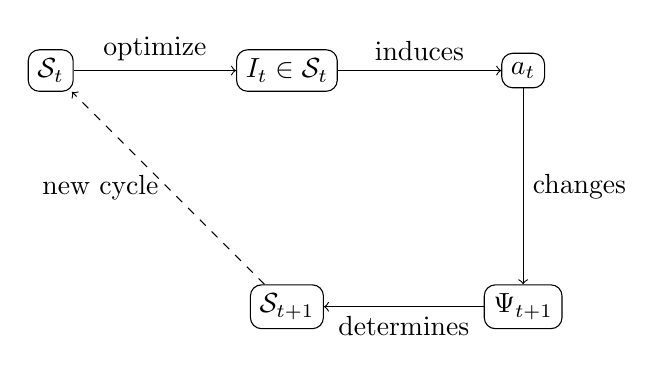
\begin{tikzpicture}[node distance=3cm, auto]
    \node[draw, rectangle, rounded corners] (S) {$\mathcal{S}_t$};
    \node[draw, rectangle, rounded corners, right of=S] (I) {$I_t \in \mathcal{S}_t$};
    \node[draw, rectangle, rounded corners, right of=I] (a) {$a_t$};
    \node[draw, rectangle, rounded corners, below of=a] (Psi) {$\Psi_{t+1}$};
    \node[draw, rectangle, rounded corners, left of=Psi] (S2) {$\mathcal{S}_{t+1}$};

    \draw[->] (S) -- node[above] {optimize} (I);
    \draw[->] (I) -- node[above] {induces} (a);
    \draw[->] (a) -- node[right] {changes} (Psi);
    \draw[->] (Psi) -- node[below] {determines} (S2);
    \draw[->, dashed] (S2) -- node[left] {new cycle} (S);
\end{tikzpicture}
\caption{The Solution Space Evolution Cycle}
\end{figure}

\begin{theorem}[Solution Space Evolution (SS-T1)]
The solution space evolves according to:
\begin{equation}
\mathcal{S}_{t+1} = \mathcal{S}\left(f(\Psi_t, h(I_t, S_t)), g(S_t, I_t, \Psi_t)\right)
\end{equation}
where $h: \mathcal{I} \times \mathcal{S} \to \mathcal{A}$ maps interventions to behavior.
\end{theorem}

\subsection{Expansion and Contraction}

Solution spaces can expand or contract:

\begin{definition}[Space Expansion]
$\mathcal{S}_{t+1} \supseteq \mathcal{S}_t$ when intervention creates enabling context.
\end{definition}

\begin{definition}[Space Contraction]
$\mathcal{S}_{t+1} \subset \mathcal{S}_t$ when intervention creates constraining context.
\end{definition}

\begin{example}[Expansion through Awareness]
An awareness intervention increases $A$:
\begin{itemize}
    \item $t$: $A = 0.2 \Rightarrow \mathcal{S}_{WHAT}$ limited (low understanding)
    \item $t+1$: $A = 0.7 \Rightarrow \mathcal{S}_{WHAT}$ expanded (can address more dimensions)
\end{itemize}
Higher awareness enables addressing previously inaccessible WHAT dimensions.
\end{example}

\begin{example}[Contraction through Reactance]
A mandating intervention triggers reactance:
\begin{itemize}
    \item $t$: $\Psi_{autonomy}$ high $\Rightarrow \mathcal{S}_{READY}$ includes nudges
    \item $t+1$: Reactance triggered $\Rightarrow \mathcal{S}_{READY}$ contracts (resistance to further intervention)
\end{itemize}
Over-intervention can shrink future solution spaces.
\end{example}

%% ============================================================================
%% SECTION 6: MULTI-EQUILIBRIA NAVIGATION
%% ============================================================================
\section{Multi-Equilibria Navigation}
\label{sec:ss-equilibria}

\subsection{Equilibrium Basins within Solution Space}

From Chapter 7 and Axiom SS-A7, complementarity creates multiple equilibria. Within $\mathcal{S}$, we can identify equilibrium basins:

\begin{definition}[Equilibrium Basin]
$\mathcal{E}_i \subset \mathcal{S}$ is an equilibrium basin if:
\begin{equation}
\forall I \in \mathcal{E}_i: \text{gradient descent from } I \text{ converges to } I^*_i
\end{equation}
\end{definition}

\begin{theorem}[Basin Structure (SS-T2)]
For complementarity matrix $\Gamma$ with $\gamma_{ij} > 0$, the number of equilibrium basins is:
\begin{equation}
|\{\mathcal{E}_i\}| \geq 2^{|\{(i,j): \gamma_{ij} > \gamma_{crit}\}|}
\end{equation}
Strong complementarity creates exponentially many potential equilibria.
\end{theorem}

\subsection{The Valley Problem Formalized}

\begin{theorem}[Valley Crossing (SS-T3)]
If $I^*_1 \in \mathcal{E}_1$ and $I^*_2 \in \mathcal{E}_2$ are equilibria in different basins with $P_{eff}(I^*_2) > P_{eff}(I^*_1)$, then either:
\begin{enumerate}
    \item Direct path exists: $\exists$ path $p: [0,1] \to \mathcal{S}$ with $p(0) = I^*_1, p(1) = I^*_2$
    \item Valley crossing required: The minimum path passes through $I$ with $P_{eff}(I) < P_{eff}(I^*_1)$
    \item Context change required: $\nexists$ path in $\mathcal{S}(\Psi_t)$, but $\exists$ path in $\mathcal{S}(\Psi')$ for some $\Psi' \neq \Psi_t$
\end{enumerate}
\end{theorem}

Case 3 is the key insight: \textbf{changing context can create paths that don't exist in current context}.

\subsection{Context-Enabled Transitions}

\begin{corollary}[Context as Path Creator]
If transition $I^*_1 \to I^*_2$ is blocked in $\mathcal{S}(\Psi_t)$, there may exist intervention sequence $\{I_\tau\}_{\tau=t}^{t+k}$ such that:
\begin{equation}
I_t \to \Psi_{t+1} \to I_{t+1} \to \cdots \to \Psi_{t+k} \to I^*_2 \in \mathcal{S}(\Psi_{t+k})
\end{equation}
The path requires \textbf{sequential context modification} rather than direct transition.
\end{corollary}

This formalizes the ``EMERGE creates new possibilities'' insight: interventions that change context can enable future interventions that were previously infeasible.

%% ============================================================================
%% SECTION 7: RESULTS - KEY PROPERTIES
%% ============================================================================
\section{Results: Key Properties of Solution Spaces}
\label{sec:ss-results}

\subsection{Convexity and Non-Convexity}

\begin{theorem}[Non-Convexity from Complementarity (SS-T4)]
If $\gamma_{ij} > 0$ for some $(i,j)$, then $\mathcal{S}(\Psi, S)$ is generally non-convex:
\begin{equation}
\gamma_{ij} > 0 \Rightarrow \exists I_1, I_2 \in \mathcal{S}: \lambda I_1 + (1-\lambda) I_2 \notin \mathcal{S} \text{ for some } \lambda \in (0,1)
\end{equation}
\end{theorem}

\textbf{Implication:} Linear interpolation between feasible interventions may be infeasible. Complementarity creates ``holes'' in the solution space.

\subsection{Boundary Characterization}

The boundary $\partial \mathcal{S}$ consists of:
\begin{enumerate}
    \item \textbf{Hard constraints}: Physical/logical impossibilities
    \item \textbf{Context constraints}: Current-context limitations (can change)
    \item \textbf{Complementarity constraints}: Cross-dimensional requirements
\end{enumerate}

\begin{equation}
\partial \mathcal{S} = \partial \mathcal{S}_{hard} \cup \partial \mathcal{S}_{context} \cup \partial \mathcal{S}_{compl}
\end{equation}

Only $\partial \mathcal{S}_{context}$ and $\partial \mathcal{S}_{compl}$ can shift through intervention.

\subsection{Volume Dynamics}

Define solution space volume:
\begin{equation}
V(\mathcal{S}) = \int_{\mathcal{S}} dI
\end{equation}

\begin{proposition}[Volume Conservation Failure]
In general, $V(\mathcal{S}_{t+1}) \neq V(\mathcal{S}_t)$. Interventions can increase or decrease total feasible options.
\end{proposition}

This has profound implications: \textbf{acting now may expand or contract future possibilities}.

%% ============================================================================
%% SECTION 8: IMPLICATIONS
%% ============================================================================
\section{Implications}
\label{sec:ss-implications}

\subsection{For Practitioners}

\begin{enumerate}
    \item \textbf{Feasibility First}: Before optimizing $P_{eff}$, characterize $\mathcal{S}(\Psi, S)$
    \item \textbf{Space Expansion Strategy}: Some interventions are valuable because they expand future $\mathcal{S}$, not because they maximize current $P_{eff}$
    \item \textbf{Valley Awareness}: Recognize when superior equilibria require context change, not direct intervention
    \item \textbf{Sequence Matters}: The order of interventions affects which solution spaces become accessible
\end{enumerate}

\subsection{For Researchers}

\begin{enumerate}
    \item \textbf{Endogenous Constraints}: Model how intervention changes the constraint set, not just outcomes
    \item \textbf{Dynamic Feasibility}: Study how $\mathcal{S}_t \to \mathcal{S}_{t+1}$ transitions enable or block intervention paths
    \item \textbf{Complementarity Topology}: Map the equilibrium basin structure for specific domains
\end{enumerate}

\subsection{For Policy Makers}

\begin{enumerate}
    \item \textbf{Context Policy}: Some policies work by expanding solution spaces (enabling) rather than directly changing behavior
    \item \textbf{Path Dependency}: Early interventions shape which future interventions become feasible
    \item \textbf{Lock-In Risk}: Contracting solution spaces can create irreversible constraints
\end{enumerate}

%% ============================================================================
%% SECTION 9: WORKED EXAMPLE
%% ============================================================================
\section{Worked Example: Retirement Savings Intervention}
\label{sec:ss-example}

Consider designing interventions to increase retirement savings. We trace how the solution space evolves through a sequence of interventions.

\subsection{Initial State and Context}

\textbf{State $S_0$:}
\begin{itemize}
    \item $A = 0.2$ (low awareness of retirement needs)
    \item $W = 0.3$ (low willingness to save)
    \item $\phi = $ Contemplation (early BCJ stage)
    \item $\gamma_{WHAT,HOW} = 0.4$ (financial and commitment are complementary)
\end{itemize}

\textbf{Context $\Psi_0$:}
\begin{itemize}
    \item $\Psi_{default} = $ opt-in (must actively choose to save)
    \item $\Psi_{attention} = $ low (competing financial priorities)
    \item $\Psi_{peer} = $ weak (no visible peer saving behavior)
\end{itemize}

\subsection{Initial Solution Space $\mathcal{S}_0$}

Given low awareness ($A = 0.2$), the AWARE dimension constraints limit complex interventions:
\begin{equation}
\mathcal{S}_{AWARE,0} = \{I_{AWARE} : I_{AWARE} \leq 0.4\}
\end{equation}
Only simple awareness interventions are feasible (complex financial education would not be absorbed).

Given opt-in default, the WHEN dimension is constrained:
\begin{equation}
\mathcal{S}_{WHEN,0} = \{I_{WHEN} : \text{no automatic enrollment feasible}\}
\end{equation}

Given complementarity $\gamma_{WHAT,HOW} = 0.4$, a coupling constraint applies:
\begin{equation}
|I_{WHAT,F} - I_{HOW}| \leq 0.3
\end{equation}
Financial incentives and commitment devices must move together.

\textbf{Feasible interventions in $\mathcal{S}_0$:}
\begin{enumerate}
    \item Simple information campaigns ($I_{AWARE} = 0.3$)
    \item Basic savings prompts ($I_{WHAT,F} = 0.2$, $I_{HOW} = 0.2$)
    \item Peer comparison (limited by weak $\Psi_{peer}$)
\end{enumerate}

\textbf{Infeasible in $\mathcal{S}_0$:}
\begin{enumerate}
    \item Automatic enrollment (blocked by $\Psi_{default}$)
    \item Complex financial education (blocked by low $A$)
    \item High commitment devices alone (blocked by complementarity constraint)
\end{enumerate}

\subsection{Intervention $I_0$: Awareness Campaign}

Choose intervention: $I_0 = (I_{AWARE} = 0.35, \text{others} = 0)$

\textbf{Effect:}
\begin{itemize}
    \item Behavior: Some employees attend information sessions
    \item State change: $A: 0.2 \to 0.5$
    \item Context change: $\Psi_{attention}: \text{low} \to \text{medium}$
\end{itemize}

\subsection{Evolved Solution Space $\mathcal{S}_1$}

With higher awareness ($A = 0.5$), new interventions become feasible:
\begin{equation}
\mathcal{S}_{AWARE,1} = \{I_{AWARE} : I_{AWARE} \leq 0.7\}
\end{equation}

The solution space has \textbf{expanded}:
\begin{itemize}
    \item Financial education programs now feasible
    \item More sophisticated commitment devices accessible
    \item $V(\mathcal{S}_1) > V(\mathcal{S}_0)$
\end{itemize}

\subsection{Intervention $I_1$: Commitment + Matching}

Now choose: $I_1 = (I_{WHAT,F} = 0.4, I_{HOW} = 0.5)$

This satisfies the complementarity constraint ($|0.4 - 0.5| = 0.1 \leq 0.3$) and is now feasible because awareness increased.

\textbf{Effect:}
\begin{itemize}
    \item Behavior: Employees sign up for matched savings with commitment
    \item State change: $W: 0.3 \to 0.6$, $\phi: $ Contemplation $\to$ Preparation
    \item Context change: $\Psi_{peer}: \text{weak} \to \text{medium}$ (visible peer participation)
\end{itemize}

\subsection{Solution Space $\mathcal{S}_2$: Expanded Further}

With $\phi = $ Preparation and stronger peer context:
\begin{equation}
\mathcal{S}_{STAGE,2} = \{I_{STAGE} : \text{Action-phase interventions now feasible}\}
\end{equation}

New interventions become possible:
\begin{enumerate}
    \item Social norm messaging (enabled by $\Psi_{peer}$)
    \item Automatic escalation (Preparation stage allows)
    \item Goal-setting workshops (sufficient $W$)
\end{enumerate}

\subsection{The Valley Problem}

Suppose the superior equilibrium $I^*_2$ requires automatic enrollment (default change). This is \textbf{still infeasible} in $\mathcal{S}_2$ because $\Psi_{default}$ hasn't changed.

To reach $I^*_2$, we need a \textbf{policy intervention} that changes $\Psi_{default}$:
\begin{equation}
\text{Policy} \to \Psi_{default}: \text{opt-in} \to \text{opt-out} \to \mathcal{S}_3 \ni I^*_2
\end{equation}

This illustrates SS-A8 (Valley Problem): the direct path to the best equilibrium doesn't exist in current solution space; context must change first.

\subsection{Summary Table}

\begin{center}
\begin{tabular}{|l|c|c|c|c|}
\hline
\textbf{Time} & \textbf{Intervention} & \textbf{Key State Change} & \textbf{Context Change} & \textbf{Space Change} \\
\hline
$t=0$ & --- & --- & --- & $\mathcal{S}_0$ (narrow) \\
$t=1$ & Awareness & $A: 0.2 \to 0.5$ & $\Psi_{attn}\uparrow$ & Expand \\
$t=2$ & Commit+Match & $W: 0.3 \to 0.6$ & $\Psi_{peer}\uparrow$ & Expand \\
$t=3$ & Policy & --- & $\Psi_{default}$ & Enable $I^*_2$ \\
\hline
\end{tabular}
\end{center}

This worked example demonstrates:
\begin{enumerate}
    \item Solution space is context-dependent ($\mathcal{S}_0 \neq \mathcal{S}_1 \neq \mathcal{S}_2$)
    \item Interventions expand future possibilities (space expansion)
    \item Complementarity constrains intervention combinations
    \item Superior equilibria may require context change (valley problem)
    \item Sequencing matters (awareness first enables later interventions)
\end{enumerate}

%% ============================================================================
%% SECTION 10: CONNECTION TO MP OPTIMIZATION
%% ============================================================================
\section{Connection to Master Optimization Problem}
\label{sec:ss-mp-connection}

Appendix UNMAPPED_MP defines the optimization:
\begin{equation}
\max_{\{I_t, P_t\}_{t=0}^T} \sum_{t=0}^{T} \delta^t \cdot P_{eff}(S_t, I_t, \Psi_t)
\end{equation}

This appendix specifies the constraint set. The complete formulation is:

\begin{equation}
\boxed{
\max_{\{I_t\}} \sum_{t=0}^{T} \delta^t \cdot P_{eff}(S_t, I_t, \Psi_t) \quad \text{s.t.} \quad I_t \in \mathcal{S}(\Psi_t, S_t) \; \forall t
}
\end{equation}

The solution space provides the \textbf{feasibility constraint} at each time step, and this constraint itself evolves endogenously.

\subsection{Bellman Equation with Solution Space}

The Bellman equation from MP becomes:
\begin{equation}
V(S_t, \Psi_t) = \max_{I_t \in \mathcal{S}(\Psi_t, S_t)} \left\{ P_{eff}(S_t, I_t, \Psi_t) + \delta \cdot \mathbb{E}[V(S_{t+1}, \Psi_{t+1})] \right\}
\end{equation}

The solution space constraint $I_t \in \mathcal{S}(\Psi_t, S_t)$ is now explicit.

%% ============================================================================
%% SECTION 10: CRITICAL FOUNDATIONS
%% ============================================================================
\section{Critical Foundations}
\label{sec:ss-foundations}

\begin{enumerate}
    \item \textbf{Chapter 7 (Non-Concavity)}: Multiple equilibria from complementarity
    \item \textbf{Chapter 9 (Context)}: $\Psi_{t+1} = f(\Psi_t, a_t)$ dynamics
    \item \textbf{Appendix UNMAPPED_MP (Master Problem)}: Objective function and state evolution
    \item \textbf{Appendix UNMAPPED_IE (EMERGE)}: Algorithm for computing interventions
    \item \textbf{Appendix UNMAPPED_V (WHEN)}: Context dimensions that determine boundaries
    \item \textbf{Appendix UNMAPPED_B (HOW)}: Complementarity structure creating coupling
\end{enumerate}

%% ============================================================================
%% SECTION 11: SUMMARY
%% ============================================================================
\section{Summary}
\label{sec:ss-summary}

This appendix formalizes the \textbf{Solution Space} $\mathcal{S}(\Psi, S)$ as the feasible region for behavioral interventions within the EBF framework.

\textbf{Key contributions:}

\begin{enumerate}
    \item \textbf{Solution Space Definition}: $\mathcal{S}(\Psi, S)$ is the set of feasible interventions given context $\Psi$ and state $S$, derived from the full intervention space $\mathcal{I} = [0,1]^9$ through constraint application.

    \item \textbf{Dimension Decomposition}: The solution space decomposes into dimension-specific components $\mathcal{S}_k$ for each 10C dimension (WHO, WHAT, HOW, WHEN, WHERE, AWARE, READY, STAGE, HIERARCHY), with complementarity creating cross-dimensional coupling constraints.

    \item \textbf{Dynamic Evolution}: The solution space evolves endogenously through the cycle $\mathcal{S}_t \to I_t \to a_t \to \Psi_{t+1} \to \mathcal{S}_{t+1}$. Interventions change context, which changes the feasible set for future interventions.

    \item \textbf{Expansion and Contraction}: Solution spaces can expand (enabling interventions) or contract (constraining interventions). Strategic planning must consider not just current $P_{eff}$ but future $\mathcal{S}$ expansion.

    \item \textbf{Multi-Equilibria Structure}: Complementarity creates multiple equilibrium basins within $\mathcal{S}$. The Valley Problem (SS-A8) formalizes that superior equilibria may only be reachable through context change, not direct intervention.

    \item \textbf{EMERGE Integration}: The EMERGE algorithm from Appendix UNMAPPED_IE is reinterpreted as a solution space generator that computes $\mathcal{S}(\Psi, S)$ from context and state.

    \item \textbf{MP Connection}: This appendix provides the constraint set for the optimization problem in Appendix UNMAPPED_MP, completing the formal optimization framework with: $\max P_{eff}$ subject to $I_t \in \mathcal{S}(\Psi_t, S_t)$.
\end{enumerate}

\textbf{Core equation:}
\begin{equation}
\mathcal{S}(\Psi, S) = \{I \in [0,1]^9 : g_j(I, \Psi, S) \leq 0, \forall j\} = \bigcap_{k=1}^{9} \mathcal{S}_k(\Psi_k, S_k)
\end{equation}

\textbf{Practical insight:} What interventions are feasible depends on where you are (context) and where you've been (state). Changing context through behavior creates new possibilities -- the solution space is not static but emerges from the intervention-behavior-context cycle.

%% ============================================================================
%% SECTION 12: OPEN ISSUES
%% ============================================================================
\section{Open Issues}
\label{sec:ss-open}

\begin{enumerate}
    \item \textbf{Computational Complexity}: How to efficiently compute $\mathcal{S}(\Psi, S)$ for high-dimensional problems?

    \item \textbf{Uncertainty in Boundaries}: How to handle uncertain context $\Psi$ leading to probabilistic solution spaces?

    \item \textbf{Learning the Transition Operator}: Can $T$ be learned from data rather than specified?

    \item \textbf{Optimal Space Expansion}: What is the optimal trade-off between current $P_{eff}$ and future $\mathcal{S}$ expansion?

    \item \textbf{Robustness}: How sensitive is $\mathcal{S}$ to small perturbations in $\Psi$?

    \item \textbf{Empirical Validation}: Methods to estimate solution space boundaries from observational data?
\end{enumerate}

%% ============================================================================
%% SECTION 12: GLOSSARY
%% ============================================================================
\section{Glossary}
\label{sec:ss-glossary}

For comprehensive definitions, see Appendix G (Glossary). Key terms for this appendix:

\begin{description}
    \item[Solution Space $\mathcal{S}(\Psi, S)$] The set of feasible interventions given context and state
    \item[Equilibrium Basin $\mathcal{E}_i$] Region of solution space converging to local optimum $I^*_i$
    \item[Transition Operator $T$] Mapping from current space and intervention to next space
    \item[Context Monotonicity] Property that enabling context expands solution space
    \item[Valley Problem] Situation where superior equilibrium requires context change for access
    \item[Space Expansion] Intervention that increases future feasible options
    \item[Space Contraction] Intervention that decreases future feasible options
\end{description}

%% ============================================================================
%% SECTION 13: REFERENCES
%% ============================================================================
\section{References}
\label{sec:ss-references}

This appendix draws on optimization theory, dynamic programming, and behavioral economics. Key foundations include constrained optimization (Boyd \& Vandenberghe), dynamic systems theory, and the EBF framework chapters.

For the complete bibliography, see the master bibliography file.

\nocite{bcm_master}

% Cross-references to other appendices
\begin{itemize}
    \item Appendix UNMAPPED_MP: Master optimization problem formulation
    \item Appendix UNMAPPED_V: Context dimensions determining solution space
    \item Appendix UNMAPPED_IE: EMERGE algorithm for intervention generation
    \item Appendix UNMAPPED_B: Complementarity creating cross-dimensional constraints
    \item Appendix UNMAPPED_AAA: WHO dimension scope constraints
    \item Appendix UNMAPPED_C: WHAT dimension utility constraints
    \item Appendix UNMAPPED_BBB: WHERE parameter constraints
\end{itemize}

\end{chapter}
